\documentclass[11pt,aspectratio=169]{beamer}
\usepackage{imaxbeamer}

\title[F21 -- 2D Randverdiproblemer]{Forelesning 21\\ To-dimensjonale randverdiproblemer og varmeligningen i 2D}
\subtitle{Kompendium §3.3.5--§3.3.6}
\author{IMAx3012 / IMAA3012 -- Matematikk 3B}
\date{}

\begin{document}

\begin{frame}
\titlepage
\end{frame}

\begin{frame}{I dag}
\begin{itemize}
\item \textbf{Forrige gang (F20):} endelige differanser i \emph{1D} -- Dirichlet- og Neumann-RVP, Jacobi/Gauss-Seidel.
\item \textbf{I dag:} samme ideer i \emph{2D}, pluss det første eksempelet på en tidsavhengig PDE:
  \begin{enumerate}
  \item To-dimensjonale randverdiproblemer: Laplace- og Poisson-ligningen (§3.3.5)
  \item Varmeligningen: semi-diskretisering og eksplisitt Euler, i 1D og 2D (§3.3.6)
  \end{enumerate}
\item \textbf{Neste gang (F22):} leapfrog-metoden for bølgeligningen -- en annen strategi for tidsavhengige PDE-er.
\end{itemize}
\end{frame}

% ======================= 3.3.5 =======================
\section{2D randverdiproblemer: Laplace og Poisson}

\begin{frame}{Poisson- og Laplace-ligningen i 2D}
Vi generaliserer 1D-RVP-et til to romdimensjoner. Poisson-ligningen (Laplace: spesialtilfellet $f=0$):
\[
\Delta u = u_{xx}+u_{yy} = f(x,y) \quad \text{i } D, \qquad u=g \quad \text{på } \partial D,
\]
på et rektangel $D=[a,b]\times[c,d]$, med gitte Dirichlet-randverdier $g$.
\begin{itemize}
\item Akkurat som i 1D: diskretiser domenet, approksimer deriverte, løs ligningssystemet.
\item Nytt: randen $\partial D$ er nå en hel \emph{kurve} (de fire kantene av rektangelet), ikke bare to endepunkter.
\end{itemize}
\end{frame}

\begin{frame}{Diskretisering: fempunktsformelen}
Rutenett $x_i=a+i\Delta x$, $y_j=c+j\Delta y$, $U_{i,j}\approx u(x_i,y_j)$. Sentraldifferanser i hver retning:
\[
\frac{U_{i-1,j}-2U_{i,j}+U_{i+1,j}}{\Delta x^2} + \frac{U_{i,j-1}-2U_{i,j}+U_{i,j+1}}{\Delta y^2} = f(x_i,y_j).
\]
\begin{center}
\begin{tikzpicture}[scale=0.9]
\foreach \x in {0,1,2} \foreach \y in {0,1,2} {\fill[black!25] (\x,\y) circle (2pt);}
\fill[thmFarge] (1,1) circle (3pt) node[below right] {\scriptsize $U_{i,j}$};
\fill[thmFarge!70] (0,1) circle (3pt) node[left] {\scriptsize $U_{i-1,j}$};
\fill[thmFarge!70] (2,1) circle (3pt) node[right] {\scriptsize $U_{i+1,j}$};
\fill[thmFarge!70] (1,0) circle (3pt) node[below] {\scriptsize $U_{i,j-1}$};
\fill[thmFarge!70] (1,2) circle (3pt) node[above] {\scriptsize $U_{i,j+1}$};
\draw[thmFarge,thick] (1,1)--(0,1) (1,1)--(2,1) (1,1)--(1,0) (1,1)--(1,2);
\end{tikzpicture}
\end{center}
Kalles \emph{fempunktsformelen} (eng. five-point stencil): kobler hvert punkt til sine fire nærmeste naboer.

I spesialtilfellet $\Delta x=\Delta y=h$:
\begin{equation}
U_{i-1,j}+U_{i+1,j}+U_{i,j-1}+U_{i,j+1} - 4U_{i,j} = h^2f(x_i,y_j).
\end{equation}
\end{frame}

\begin{frame}{Løsning: hvorfor ikke bare $A\vect U=\vect b$ direkte?}
I prinsippet: samle alle $U_{i,j}$ i én lang vektor (f.eks. radvis), sett opp fempunktsformelen som et lineært system $A\vect U=\vect b$, og løs direkte -- akkurat som i 1D.
\begin{remb}{Hvorfor er dette tungvint i 2D?}
$A$ blir en stor matrise (dimensjon = antall rutenettpunkter i hver retning, multiplisert sammen), og den eksplisitte oppbyggingen krever mye mer bokholderi enn i 1D. For store 2D-problemer er det upraktisk å sette opp hele $A$.
\end{remb}
\textbf{Løsning:} bruk Jacobi- eller Gauss-Seidel-iterasjon fra F20 -- disse generaliserer direkte, og unngår å bygge opp $A$ i det hele tatt.
\end{frame}

\begin{frame}{Jacobi/Gauss-Seidel i 2D}
Løs fempunktsformelen for $U_{i,j}$:
\begin{equation}
U_{i,j} = \frac14\Big(U_{i-1,j}+U_{i+1,j}+U_{i,j-1}+U_{i,j+1} - h^2f(x_i,y_j)\Big),
\end{equation}
og bruk dette som oppdateringsformel, akkurat som i 1D:
\begin{itemize}
\item \textbf{Jacobi:} oppdater alle $U_{i,j}$ samtidig, med verdier fra forrige iterasjon.
\item \textbf{Gauss-Seidel:} bruk oppdaterte verdier så snart de er tilgjengelige (f.eks. rad for rad).
\end{itemize}
Randpunktene $U_{i,j}$ holdes fast lik de gitte Dirichlet-verdiene $g(x_i,y_j)$ gjennom hele iterasjonen -- kun indre punkter oppdateres.
\begin{remb}{Posisjonsavhengige randbetingelser}
$g$ trenger ikke være konstant -- den kan variere langs hver vegg. Det eneste som kreves er at vi kan evaluere $g(x_i,y_j)$ i hvert randpunkt.
\end{remb}
\end{frame}

\begin{frame}[fragile]{Implementering (F21-notatbok)}
\begin{lstb}[Python -- setter Dirichlet-rand og itererer]
\begin{verbatim}
def sett_rand(U, g, x, y):
    U[0, :]  = [g(xi, y[0])  for xi in x]
    U[-1, :] = [g(xi, y[-1]) for xi in x]
    U[:, 0]  = [g(x[0],  yj) for yj in y]
    U[:, -1] = [g(x[-1], yj) for yj in y]
    return U

def jacobi_poisson2d(f, g, Lx, Ly, Nx, Ny, tol=1e-8, maxit=200_000):
    # ... sett opp rutenett, initialiser U, sett rand med sett_rand ...
    # itererer U[i,j] = 0.25*(U[i-1,j]+U[i+1,j]+U[i,j-1]+U[i,j+1] - h^2 f)
    ...
\end{verbatim}
\end{lstb}
\end{frame}

\begin{frame}{Test mot kjent løsning}
Manufactured solution: $u(x,y)=\sin(\pi x)\sin(\pi y)$ på $[0,1]^2$, $u=0$ på randen, $f=\Delta u=-2\pi^2\sin(\pi x)\sin(\pi y)$.
\begin{center}
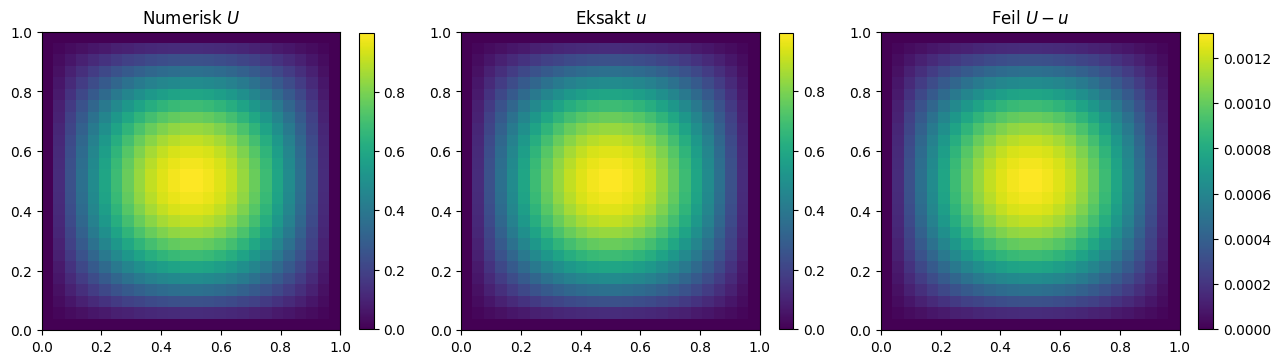
\includegraphics[width=0.95\textwidth]{assets/jacobi_test.png}
\end{center}
\end{frame}

\begin{frame}{Posisjonsavhengig (stykkevis) Dirichlet-rand}
Samme kode, men $g(x,y)$ er nå stykkevis lineær langs hver av de fire kantene -- akkurat som i øvingsoppgaver med f.eks. en temperaturfordeling langs randen av en plate.
\begin{center}
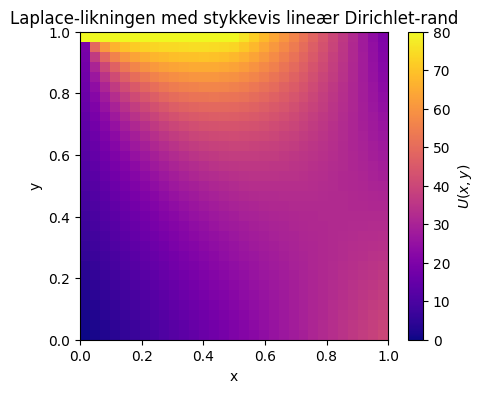
\includegraphics[width=0.75\textwidth]{assets/jacobi_piecewise.png}
\end{center}
\end{frame}

% ======================= 3.3.6 =======================
\section{Varmeligningen: semi-diskretisering}

\begin{frame}{Fra ODE-er til PDE-er}
Så langt: endelige differanser for å løse \emph{randverdiproblemer} (ODE-er i rom). Nå: samme strategi utvidet til \emph{tidsavhengige PDE-er} -- med varmeligningen som eksempel (men teknikken gjelder generelt):
\[
u_t = u_{xx}, \quad 0\le x\le 1, \qquad u(0,t)=g_0(t),\ u(1,t)=g_1(t), \qquad u(x,0)=f(x).
\]
Essensen: \emph{semi-diskretisering} -- diskretiser kun i rom, la tiden foreløpig være kontinuerlig.
\end{frame}

\begin{frame}{Semi-diskretisering: steg 1--3}
\begin{enumerate}
\item[\textbf{1.}] Diskretiser kun i $x$: $x_i=i\Delta x$, $\Delta x=1/M$. For hver $x_i$ er $u(x_i,t)$ en funksjon \emph{kun} av $t$.
\item[\textbf{2.}] Diskretiser høyresiden med sentraldifferanse (i rom, ved et vilkårlig fast $t$):
\[
\frac{\partial u}{\partial t}(x_i,t) \approx \frac{u(x_{i+1},t)-2u(x_i,t)+u(x_{i-1},t)}{\Delta x^2}.
\]
\item[\textbf{3.}] Erstatt $u(x_i,t)$ med $U_i(t)$:
\[
U_i'(t) = \frac{U_{i+1}(t)-2U_i(t)+U_{i-1}(t)}{\Delta x^2}, \quad i=1,\ldots,M-1,
\]
med $U_0(t)=g_0(t)$, $U_M(t)=g_1(t)$, $U_i(0)=f(x_i)$.
\end{enumerate}
Dette er et veldefinert \textbf{system av ODE-er} -- en \emph{semi-diskretisering} av PDE-en.
\end{frame}

\begin{frame}{Viktig presisering: hva bestemmer ordenen i tid?}
\begin{remb}{Semi-diskretisering sier ingenting om tidsordenen ennå}
Steg 1--3 diskretiserer kun i \emph{rom}. Resultatet er et system av ODE-er som i prinsippet er \emph{eksakt} i tid -- ingen tidsapproksimasjon er gjort ennå. Sentraldifferansen i rom er $O(\Delta x^2)$, men dette sier ingenting om nøyaktigheten i tid.

Nøyaktigheten i \emph{tid} avgjøres først i \textbf{steg 4}, når vi velger en konkret metode for å løse ODE-systemet.
\end{remb}
\end{frame}

\begin{frame}{Steg 4: løs ODE-systemet -- eksplisitt Euler}
For konkrethets skyld bruker vi eksplisitt Euler med tidssteg $\Delta t$:
\begin{equation}
U_i^{n+1} = U_i^n + r\big(U_{i+1}^n - 2U_i^n + U_{i-1}^n\big), \qquad r=\frac{\Delta t}{\Delta x^2},
\end{equation}
der $U_i^n\approx u(x_i,t_n)$, $t_n=n\Delta t$.
\begin{remb}{Eksplisitt Euler er kun 1. ordens i tid}
Selv om romdiskretiseringen (sentraldifferansen) er $O(\Delta x^2)$, er \emph{eksplisitt Euler selv} en \textbf{førsteordens} metode i tid -- akkurat som for ODE-er. Den totale feilen i dette skjemaet er dermed $O(\Delta t) + O(\Delta x^2)$: førsteordens i tid, andreordens i rom.
\end{remb}
\end{frame}

\begin{frame}{Stabilitet: CFL-betingelsen}
\begin{remb}{Stabilitet}
Eksplisitt Euler er \emph{ikke} ubetinget stabil: for stor $\Delta t$ i forhold til $\Delta x$ gjør at feil vokser eksponentielt. Metoden er stabil nøyaktig når
\[
r = \frac{\Delta t}{\Delta x^2} \leq \frac12.
\]
Dette er et eksempel på en \emph{CFL-betingelse} (Courant--Friedrichs--Lewy). I praksis: finere romdiskretisering ($\Delta x$ mindre) krever et \emph{mye} mindre tidssteg, siden $\Delta t\propto \Delta x^2$.
\end{remb}
\begin{center}
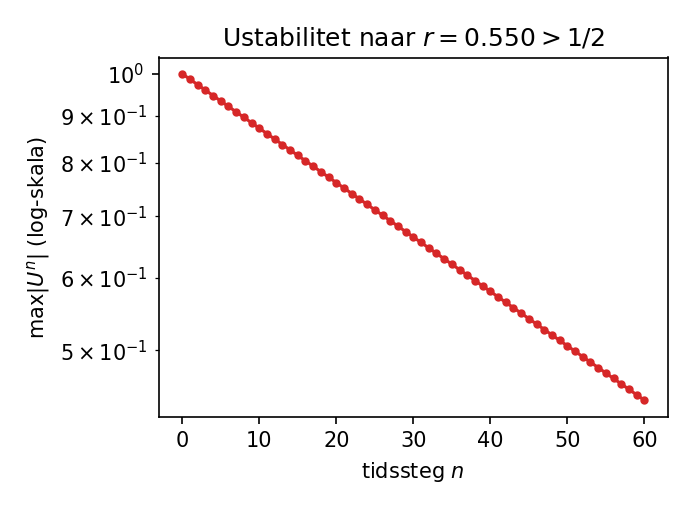
\includegraphics[width=0.55\textwidth]{assets/heat1d_ustabil.png}
\end{center}
\end{frame}

\begin{frame}{Numerisk eksempel 1: kjent eksakt løsning}
$u(x,0)=\sin(\pi x)$, $g_0=g_1=0$. Eksakt løsning: $u(x,t)=e^{-\pi^2 t}\sin(\pi x)$.
\begin{center}
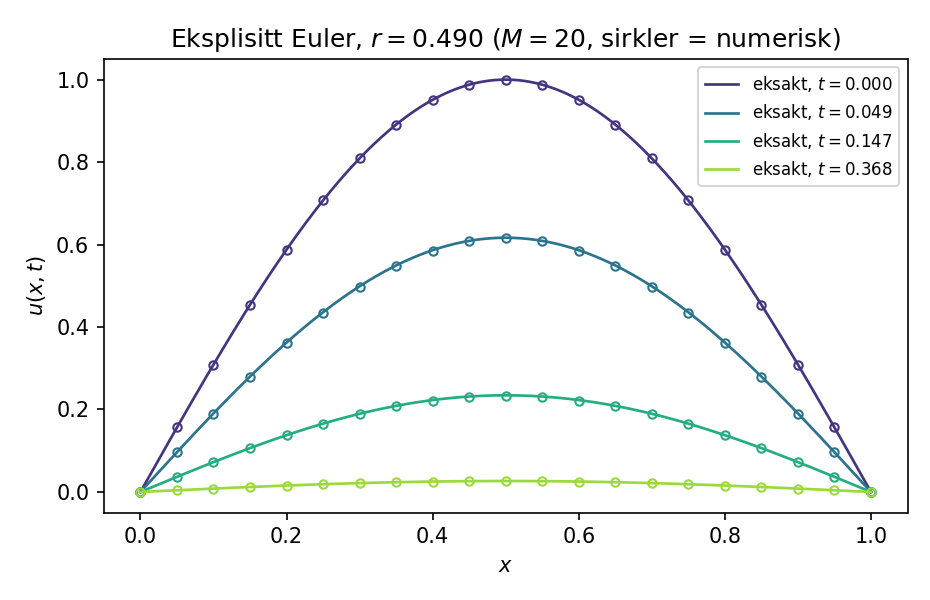
\includegraphics[width=0.85\textwidth]{assets/heat1d_eks1.png}
\end{center}
Sirkler = numerisk ($r<1/2$, stabilt), heltrukket = eksakt -- de faller sammen, og begge går mot $0$ når $t\to\infty$ (varmen jevner seg ut).
\end{frame}

\begin{frame}{Numerisk eksempel 2: hatt-funksjon}
\[
u(x,0) = \begin{cases} 2x, & 0\le x\le 0.5 \\ 2(1-x), & 0.5<x\le 1\end{cases}, \qquad g_0=g_1=0.
\]
Her er \emph{ikke} den eksakte løsningen gitt i enkel form -- vi observerer bare den numeriske løsningen glatte seg ut over tid.
\begin{center}
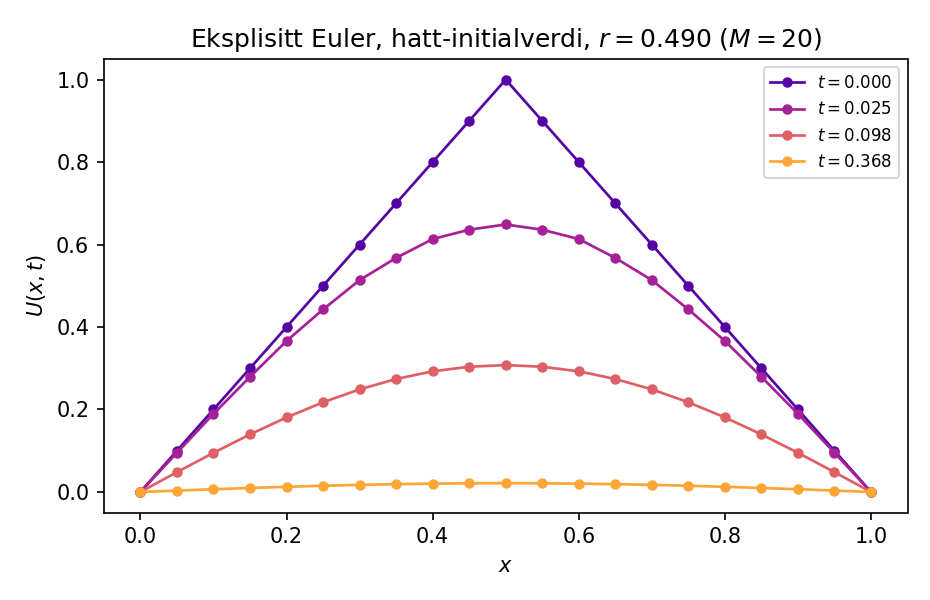
\includegraphics[width=0.78\textwidth]{assets/heat1d_eks2.png}
\end{center}
\end{frame}

\begin{frame}{Generalisering til to romdimensjoner}
Samme teknikk på $u_t=\Delta u = u_{xx}+u_{yy}$, med fempunktsformelen i rom og eksplisitt Euler i tid, $\Delta x=\Delta y=h$:
\begin{equation}
U_{i,j}^{n+1} = U_{i,j}^n + r\Big(U_{i-1,j}^n+U_{i+1,j}^n+U_{i,j-1}^n+U_{i,j+1}^n - 4U_{i,j}^n\Big), \quad r=\frac{\Delta t}{h^2},
\end{equation}
på indre punkter; randpunktene holdes fast lik gitte randverdier i hvert tidssteg.
\begin{remb}{Stabilitet i 2D}
Stabil når $r\le \dfrac14$ (og mer generelt $\frac{\Delta t}{\Delta x^2}+\frac{\Delta t}{\Delta y^2}\le\frac12$ hvis $\Delta x\neq\Delta y$) -- strengere enn i 1D.
\end{remb}
\end{frame}

\begin{frame}{2D varmeligning: stabil kjøring}
En "varm klatt" i midten av en kald plate, $r=0.24<1/4$:
\begin{center}
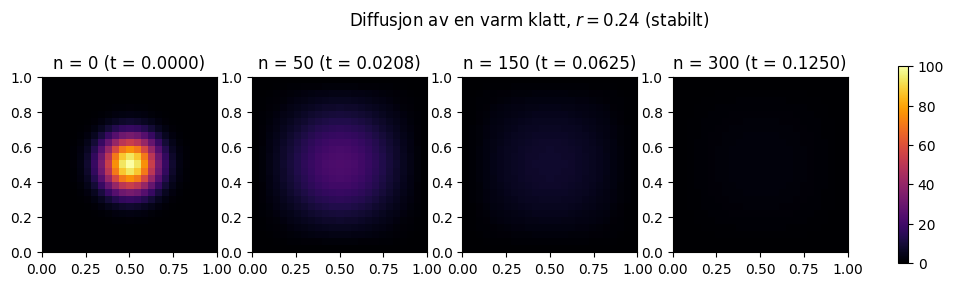
\includegraphics[width=0.95\textwidth]{assets/heat2d_stable.png}
\end{center}
\end{frame}

\begin{frame}{2D varmeligning: ustabil kjøring}
Samme problem, men $r=0.3>1/4$ -- skjemaet "eksploderer":
\begin{center}
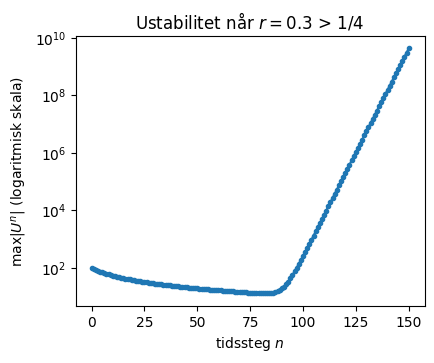
\includegraphics[width=0.55\textwidth]{assets/heat2d_unstable.png}
\end{center}
\begin{remb}{Kobling til Laplace/Poisson}
La løsningen tidsutvikle seg til den blir (tilnærmet) stasjonær, $U^{n+1}\approx U^n$ -- dette gir en tilnærming til Laplace-/Poisson-ligningen. Jacobi/Gauss-Seidel-iterasjon (tidligere i denne forelesningen) er en \emph{raskere} direkte måte å finne akkurat denne stasjonære løsningen på.
\end{remb}
\end{frame}

\begin{frame}{Oppsummering}
\begin{itemize}
\item 2D Poisson/Laplace: fempunktsformelen + Jacobi/Gauss-Seidel-iterasjon, direkte generalisering fra 1D. Randen kan være posisjonsavhengig.
\item Varmeligningen løses ved \emph{semi-diskretisering}: diskretiser i rom $\to$ ODE-system $\to$ velg en tidsintegrator.
\item Semi-diskretiseringen i seg selv sier ingenting om tidsordenen -- det er \emph{valget av ODE-metode} (her: eksplisitt Euler) som gjør skjemaet førsteordens i tid.
\item Eksplisitt Euler er betinget stabilt: $r=\Delta t/\Delta x^2\le \frac12$ i 1D, $r\le\frac14$ i 2D.
\end{itemize}
\end{frame}

\begin{frame}{Neste gang: F22 -- leapfrog-metoden}
\begin{nestefb}
Varmeligningen er \emph{førsteordens i tid}, så eksplisitt Euler (ett tidsnivå) er en naturlig start. Bølgeligningen $u_{tt}=c^2u_{xx}$ er derimot \emph{andreordens i tid} -- eksplisitt Euler passer ikke direkte.

Neste gang ser vi på \textbf{leapfrog-metoden}: en sentraldifferanse også i tid, som er \emph{bedre egnet} for denne typen problemer -- andreordens nøyaktig i tid, og uten den kunstige numeriske dempingen eksplisitt Euler ville gitt.
\end{nestefb}
\end{frame}

\end{document}
